\section{Theory}
Beta decay is commonly observed in unstable nuclei that contain an excess of neutrons compared to protons. The $\beta$ particles are typically high-energy electrons ($\beta^-$) or positrons  ($\beta^+$) that are ejected from the nucleus. These particles have a much smaller mass than a proton, making up only onehalf of one-thousandth of its mass. Despite their small mass, they can achieve high speeds close to the speed of light due to their high energy.

Because of their light mass, $\beta$ particles quickly lose energy as they interact with matter. As a result, they have limited ranges in materials, typically only a few millimeters. However, their range in air can be tens of centimeters, depending on their energy. The process of beta decay and the resulting beta radiation have important applications in various fields, including nuclear physics and medical imaging. The ability of $\beta$ particles to penetrate materials to a limited depth makes them useful in measuring material thickness and in detecting material defects. In medicine, beta-emitting radioactive isotopes are used for cancer treatment and imaging.

\subsection{Range of $\beta$ particle}
The maximum distance beta particles can travel
within a material before losing all their energy and
being completely absorbed is referred to as their
range. This range depends on both the initial kinetic energy of the beta particles and the density of the material they traverse. The endpoint energy ($E_0$)
represents the highest kinetic energy a beta particle
can have when emitted from a radioactive source, as
beta decay results in a continuous energy spectrum.
A widely used method for determining beta particle
range is the half-thickness technique, which involves
measuring the thickness of an absorber required to
reduce the detected count rate by half.

The range of $\beta$ particle is given by 
\begin{align}
    R=(0.52E_o-0.09) \text{ g/cm}^2
\end{align}
where $E_0$ is the endpoint energy of the beta rays in MeV. The ratio of thickness required to reduce the counts of beta rays from one source to half to the thickness required for the other source is given by
\begin{align}
    \frac{t_{\frac{1}{2},1}}{t_{\frac{1}{2},2}}=\frac{\text{Range of beta rays from first source}}{\text{Range of beta rays from second source}}
\end{align}
\begin{align}
    \frac{t_{\frac{1}{2},1}}{t_{\frac{1}{2},2}}=\frac{R_1}{R_2}
\end{align}

By comparing half-thickness values for different beta sources,
the range for an unknown source can be estimated.

\subsection{Back scattering}
When a $\beta$ particle, either an electron or a positron, enters a material, it undergoes a series of interactions with the atoms in the material. The attractive electrostatic force between the positively charged nucleus of the atoms and the negatively charged $\beta$ particle causes the path of the $\beta$ particle to be deflected. The degree of deflection depends on the energy of the $\beta$ particle, but the overall effect is a scattering of the particles. Typically, this causes the forward direction of the $\beta$ particle to change by a few degrees.

In some cases, however, the angle of deflection can be quite large, and the $\beta$ particle can be deflected back in the direction from which it came. This phenomenon is known as backscattering, and it occurs when the angle of deflection is greater than 90 degrees. Backscattering is more likely to occur in materials with high atomic number, as the larger number of positively charged nuclei increases the likelihood of a strong electrostatic interaction with the $\beta$ particle.

Backscattering of $\beta$ particles has important implications for radiation detection and measurement. For example, when using a detector to measure the amount of beta radiation emitted from a sample, backscattering can cause a portion of the radiation to be reflected back into the sample, leading to an overestimation of the true amount of radiation emitted. To mitigate this effect, detectors are often designed with thin windows or other features that minimize backscattering and allow the $\beta$ particles to escape from the sample more easily.

In addition to its impact on radiation detection, backscattering of $\beta$ particles also plays a role in the interactions between radiation and matter in a variety of contexts, including medical imaging and radiation therapy. Understanding the principles of backscattering is therefore important for a wide range of applications in the fields of nuclear physics, radiation biology, and radiation protection.

\subsection{Bremsstrahlung Radiation}
Bremsstrahlung is a form of electromagnetic radiation which is generated when a charged particle experiences a deacceleration by another charged particle, such as an atomic nucleus. When a $\beta$ particle moves through matter, it may encounter a nucleus and be deflected by it. This deflection causes a reduction in the $\beta$ particle's kinetic energy, resulting in the emission of energy in the form of a photon of bremsstrahlung radiation or `breaking radiation' (Fig. \ref{g1}). The energy of the emitted bremsstrahlung photon is equal to the difference in energy between the initial and final kinetic energies of the $\beta$ particle.

\begin{figure}
    \centering
    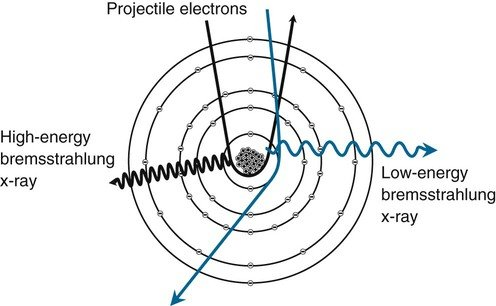
\includegraphics[width=1\columnwidth]{images/brem.jpg}
    \caption{Origin of Bremsstrahlung radiation}
    \label{g1}
\end{figure}

The amount of bremsstrahlung radiation emitted by a $\beta$ particle depends on several factors, including the kinetic energy of the $\beta$ particle, the atomic number of the absorbing material, and the density of the material. As the $\beta$ particle approaches a nucleus and is deflected, the magnitude of the deflection and the associated energy loss depend on the proximity and atomic charge of the nucleus. The closer the $\beta$ particle is to the nucleus, the greater the energy loss, and the higher the frequency of the emitted bremsstrahlung photons. In addition, the higher the atomic number of the absorbing material, the greater the number of potential nuclei that the $\beta$ particle may interact with, leading to an increased probability of bremsstrahlung radiation emission.


% ======================================================
\subsection*{Apparatus}

\begin{enumerate}
    \item Sr-90 and Th-204 samples
    \item GM counting System
    \item GM detector
    \item Sliding Bench
    \item Detector Stand
    \item Aluminium Absorber set
    \item Lead block for isolation
    \item Absorber stand for back-scattering
    \item Copper, Aluminium and Perspex plates
    \item BNC cable\\
\end{enumerate}

\begin{figure}
    \centering
    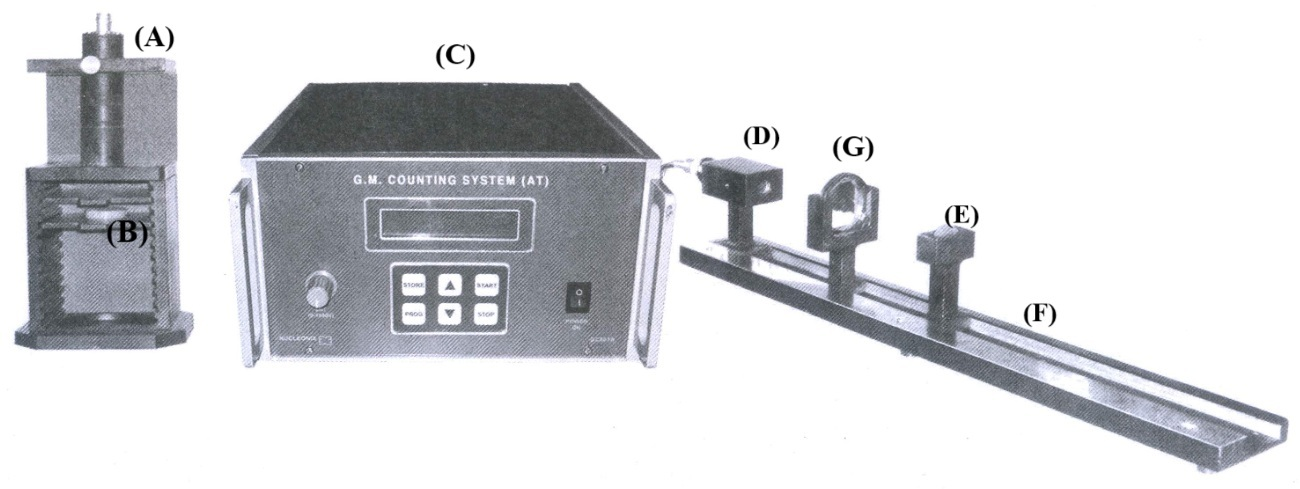
\includegraphics[width=1\columnwidth]{images/t2.jpg}
    \caption{Experimental Setup where (A) and (B) are the end window detector and source holder (C) is the GM counting system where you can vary the EHT (D) and (E) are the end window detector and source holders attached to a (E) sliding bench. (G) is the stand for the aluminium absorber set.}
    \label{t3}
\end{figure}

\begin{figure}
    \centering
    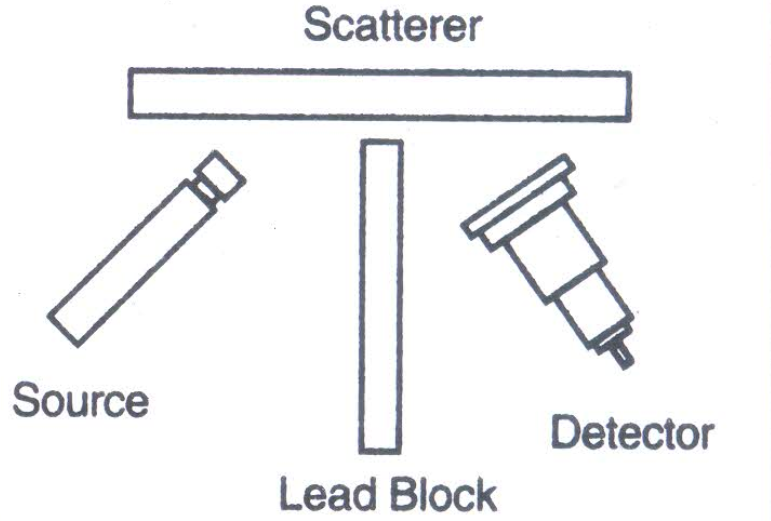
\includegraphics[width=0.7\columnwidth]{images/back.png}
    \caption{Schematic diagram for the measurement of back-scattering}
    \label{t1}
\end{figure}

\noindent Fig. \ref{t3} shows and labels the used apparatuses in this experiment. Fig. \ref{t1} shows the schamtic diagram of backscattering experiment.